\begin{problem}{1} $ $
\begin{enumerate}
	\item
	\begin{equation*}
	P(X \le 2, Y>1) = 0+\frac{1}{12}=\frac{1}{12}
	\end{equation*}
	
	\item
	
	\begin{equation*}  
  P_X(x) = \begin{cases}
                                   \frac{1}{3}+\frac{1}{12} & \text{for $x = 1$} \\
                                   \frac{1}{6}+0 & \text{for $x = 2$} \\
                                   \frac{1}{12}+\frac{1}{3} & \text{for $x = 4$} 
       \end{cases} \quad
= \begin{cases}
                                   \frac{5}{12} & \text{for $x = 1$} \\
                                   \frac{1}{6} & \text{for $x = 2$} \\
                                   \frac{5}{12} & \text{for $x = 4$} 
       \end{cases}
\end{equation*}

	\begin{equation*}  
  P_Y(y) = \begin{cases}
                                   \frac{1}{3}+\frac{1}{6}+\frac{1}{12} & \text{for $y = 1$} \\
                                   \frac{1}{12}+0+\frac{1}{3} & \text{for $y = 2$} 
       \end{cases} \quad
= \begin{cases}
                                   \frac{7}{12} & \text{for $y = 1$} \\
                                   \frac{5}{12} & \text{for $y = 2$} 
       \end{cases}
\end{equation*}

\item

	\begin{equation*}
	P(Y=2 |X=1) = \frac{P(Y=2, X=1)}{P(X=1)}=\frac{\frac{1}{12}}{\frac{5}{12}}=\frac{1}{5}
	\end{equation*}

	\begin{equation*}
	P(Y=2 |X=1) =\frac{1}{5} \neq P(Y=2) = \frac{5}{12}
	\end{equation*}
	$\implies$ not independent
	


\end{enumerate}
\end{problem}





\begin{problem}{2} $ $
\begin{enumerate}

\item The ranges of $X$, $Y$ and $Z$ are: $R_X=\{1, 2, 4 \}$, $R_Y=\{1, 2\}$ and  $R_X=\{-3, -2, -1, 0, 2\}$.  The mapping $g(x, y)=x-2y$ (where $g:R_X \times R_Y \rightarrow R_Z$) is explicitly given by:
\begin{align*}
(1, 1)& \rightarrow -1 \\
(1, 2)& \rightarrow -3 \\
(2, 1)& \rightarrow ~~0 \\
(2, 2)& \rightarrow -2 \\
(4, 1)& \rightarrow ~~2 \\
(4, 2)& \rightarrow ~~0.
\end{align*}

Thus we have the following:

	\begin{align*}  
  P_Z(z) &= \begin{cases}
                                  P(X-2Y=-3)& \text{for $z = -3$} \\
                                  P(X-2Y=-2)& \text{for $z = -2$} \\
                                  P(X-2Y=-1)& \text{for $z = -1$} \\
                                  P(X-2Y=0)& \text{for $z = 0$} \\
                                  P(X-2Y=2)& \text{for $z = 2$} 
       \end{cases} \\
&= \begin{cases}
                                  P_{XY}(1, 2) & \text{for $z = -3$} \\
                                  P_{XY}(2, 2) & \text{for $z = -2$} \\
                                  P_{XY}(1, 1) & \text{for $z = -1$} \\
                                  P_{XY}(2, 1)+P_{XY}(4, 2) & \text{for $z = 0$} \\
                                  P_{XY}(4, 1) & \text{for $z = 2$} 
       \end{cases}\\
      & = \begin{cases}
                                  \frac{1}{12} & \text{for $z = -3$} \\
                                  0 & \text{for $z = -2$} \\
                                  \frac{1}{3} & \text{for $z = -1$} \\
                                  \frac{1}{2} & \text{for $z = 0$} \\
                                  \frac{1}{12} & \text{for $z = 2$},
		\end{cases}
\end{align*}
which, as a sanity check, add up to 1.

\item 
\begin{align*}
P(X=2|Z=0) & = P(X=2|X-2Y=0) \\
 & = P(X=2|X=2Y) \\
  & = \frac{P(X=2, X=2Y)}{P(X=2Y)} \\
    & = \frac{P(X=2, Y=1)}{P(X=2, Y=1)+P(X=4, Y=2)} \\
    & = \frac{1}{3}
\end{align*}

\end{enumerate}
\end{problem}

\begin{problem}{3}
Let $A$ be the event that the first coin we pick is the fair coin.  We can find the joint PMF by conditioning on this event, and realizing that once conditioned, $X$ and $Y$ are independent (i.e., $X$ and $Y$ are conditionally independent given $A$):
\begin{align*}
P_{XY}(x, y) &= P(X=x, Y=y|A)P(A)+P(X=x, Y=y|A^c)P(A^c) \\
&= P_{1/2}(x) P_{2/3}(y)\left(\frac{1}{2}\right)+P_{2/3}(x) P_{1/2}(y)\left(\frac{1}{2}\right),
\end{align*}
where $P_{p}(z)$ is the PMF associated with a $Bern(p)$ trial.  This PMF can be written conveniently as $P_{p}(z)=p^z(1-p)^{1-z}$, so that the joint PMF is
\begin{equation*}
P_{XY}(x, y) = \left( \frac{1}{2} \right)^2 \left( \frac{2}{3} \right)^y \left( \frac{1}{3} \right)^{1-y}+\left( \frac{1}{2} \right )^2 \left( \frac{2}{3} \right)^x \left( \frac{1}{3}\right)^{1-x}.
\end{equation*}
This can also be written in tabular form as:

\begin{center}
\bgroup
\def\arraystretch{2.5}
  \begin{tabular}{ | c | c | c |}
    \hline
     & $Y=0$ & $Y=1$ \\  \hline
    $X=0$ &$\frac{1}{6}$ & $\frac{1}{4}$ \\ \hline
    $X=1$ & $\frac{1}{4}$ & $\frac{1}{3}$ \\
    \hline
  \end{tabular}
  \egroup
\end{center}
\end{problem}
To check if $X$ and $Y$ are independent I first check $(x, y)=(0,0)$.  Adding the table horizontally and vertically, the marginalized PMFs at these values are $P_X(0) = 5/12$ and $P_Y(0) = 5/12$, and thus $P_X(0)P_Y(0) = 25/144 \neq 1/6$, so $X$ and $Y$ are not independent.

\begin{problem}{4} $ $
\begin{enumerate}
\item  I first find the marginalized PMFs:

\begin{align*}
P_X(k) &= \sum_{l=1}^\infty \frac{1}{2^{k+l}} \\
&= \frac{1}{2^k}\left [-1 +  \sum_{l=0}^\infty \left(\frac{1}{2}\right)^l \right] \\
&=\frac{1}{2^k},
\end{align*}
and by symmetry
\begin{equation*}
P_Y(l)=\frac{1}{2^l},
\end{equation*}
We then have that:
\begin{align*}
P_{XY}(k, l) &= \frac{1}{2^{k+l}} \\
&= \frac{1}{2^k 2^l} \\
&= \frac{1}{2^k}\cdot \frac{1}{2^l} \\
&= P_X(k)P_Y(l) ~~\forall ~(k, l) \in \mathbb N \times \mathbb N,
\end{align*}
and thus $X$ and $Y$ are independent.

\item We can easily enumerate all pairs of $(x, y)$ that satisfy this inequality:
\begin{align*}
P(X^2+Y^2 \le 10) &= P_{XY}(1, 1)+P_{XY}(1, 2)+P_{XY}(1, 3)+P_{XY}(2, 1)+P_{XY}(2, 2)+P_{XY}(3, 1) \\
& =\frac{1}{2\cdot 2}+\frac{1}{2\cdot 2^2}+\frac{1}{2\cdot 2^3}+\frac{1}{2^2\cdot 2}+\frac{1}{2^2\cdot 2^2}+\frac{1}{2^3\cdot 2} \\
& = \frac{11}{16}.
\end{align*}

\end{enumerate}
\end{problem}

\begin{problem}{5} $ $
\begin{enumerate}

\item 


	\begin{equation*}  
  P_{X|Y}(x|1) = \begin{cases}
                                   \frac{\frac{1}{3}}{\frac{1}{3}+\frac{1}{6}+\frac{1}{12}} & \text{for $x = 1$} \\
                                   \frac{\frac{1}{6}}{\frac{1}{3}+\frac{1}{6}+\frac{1}{12}}& \text{for $x = 2$} \\
                                   \frac{\frac{1}{12}}{\frac{1}{3}+\frac{1}{6}+\frac{1}{12}} & \text{for $x = 4$} 
       \end{cases} \quad
= \begin{cases}
                                   \frac{4}{7} & \text{for $x = 1$} \\
                                    \frac{2}{7} & \text{for $x = 2$} \\
                                   \frac{1}{7} & \text{for $x = 4$} 
       \end{cases}
\end{equation*}

\item

\begin{equation*}
E[X|Y=1] = (1)\cdot \frac{4}{7}+(2)\cdot \frac{2}{7}+(4)\cdot \frac{1}{7} = \frac{12}{7}
\end{equation*}

\item

\begin{equation*}
Var[X|Y=1] = \left(1-\frac{12}{7}\right)^2\cdot \frac{4}{7}+\left(2-\frac{12}{7}\right)^2\cdot \frac{2}{7}+\left(4-\frac{12}{7}\right)^2\cdot \frac{1}{7} = \frac{52}{49}
\end{equation*}


\end{enumerate}
\end{problem}


\begin{problem}{6}  We know that $X\sim Pois(10)$ and since each customer is female independent of the other customers, if the total number of customers in an hour is $n$, then the total number of female customers in an hour is the sum of $n$ independent Bernoulli random variables.  In other words, $Y|X=n \sim Bin(n, 3/4)$.  Therefore, the joint PMF is:

\begin{align*}
P(X=n, Y=y) &= P(Y=y|X=n)P(X=n) \\
& = \binom{n}{y}\left ( \frac{3}{4} \right)^y \left ( \frac{1}{4} \right)^{n-y} \frac{10^n e^{-10}}{n!}.
\end{align*}

\end{problem}



\begin{problem}{7} We know that for a $Geom(p)$ distribution the mean is $1/p$ and the variance is $(1-p)/p^2$, so we should expect these answers.  We can find the mean by conditioning on the first ``toss":
\begin{align*}
E[X] &= E[X|H]p(H)+E[X|H^c]p(H^c) \\
&= 1\cdot p+(1+E[X])(1-p),
\end{align*}
where $E[X|H]=1$ since if we know the first toss is a heads, the experiment is done so that the mean is 1, and $E[X|H^c] =(1+E[X])$ since if the first toss is a tails, then we've wasted 1 toss, and since the geometric distribution is memoryless, it starts over at the next toss.  Solving this equation for $E[X]$ we find that $E[X] =1/p$, which is what we expected.

We can solve for $E[X^2]$ in a similar manner:
\begin{align*}
E[X^2] &= E[X^2|H]p(H)+E[X^2|H^c]p(H^c) \\
&= 1\cdot p+E[(1+X)^2](1-p) \\
&= p+E[X^2](1-p)+2E[X](1-p)+(1-p),
\end{align*}
where $E[X^2|H]=1$ for the same reason as above, and $E[X^2|H^c] = E[(1+X)^2]$ since, as above, we've wasted 1 toss on the first toss, and then the experiment starts over on the second.  Solving this equation, I find $E[X^2] = (2-p)/p^2$.  The variance is thus: $Var[X] = E[X^2]-E[X]^2 = (1-p)/p^2$, which is what we expected.

\end{problem}

\begin{problem}{8} If $X, Y\distas{iid} Geom(p)$, the we can easily find the joint PMF and use LOTUS to solve for the expectation.  The joint PMF is:
\begin{equation}
P_{XY} (x,y) = P_X(x)P_Y(y) = p(1-p)^{x-1}p(1-p)^{y-1} ~~\mathrm{for}~x, y =1, 2, \ldots,
\end{equation}
where I have multiplied the marginal PMFs since $X$ and $Y$ are independent.  Using LOTUS:

\begin{align*}
E\left [ \frac{X^2+Y^2}{XY}\right] &= \sum_{x=1}^\infty \sum_{y=1}^\infty \left( \frac{x^2+y^2}{xy}\right)p(1-p)^{x-1}p(1-p)^{y-1} \\
& = \sum_{x=1}^\infty \sum_{y=1}^\infty \frac{x}{y}p(1-p)^{x-1}p(1-p)^{y-1} +\sum_{y=1}^\infty \sum_{x=1}^\infty \frac{y}{x}p(1-p)^{x-1}p(1-p)^{y-1} \\
& = 2\sum_{x=1}^\infty \sum_{y=1}^\infty \frac{x}{y}p(1-p)^{x-1}p(1-p)^{y-1} \\
& = 2\sum_{x=1}^\infty x p(1-p)^{x-1} \sum_{y=1}^\infty \frac{1}{y}p(1-p)^{y-1},
\end{align*}
where going from the second to third line we realize that due to the symmetry, both of the sums are the same.  In the last line the first sum is just the mean of a $Geom(p)$ distribution ($1/p$).  We can simplify the second sum by utilizing the following Taylor expansion:

\begin{equation*}
- \ln (1-x)= \sum_{k=1}^\infty \frac{x^k}{k}~~ \mathrm{for}~|x|<1.
\end{equation*}
Thus, we arrive at:
\begin{align*}
E\left [ \frac{X^2+Y^2}{XY}\right] & = \frac{2}{p}p(1-p)^{-1} (-\ln p) \\
& = \frac{2}{1-p} \ln \left(\frac{1}{p} \right).
\end{align*}
\end{problem}

\begin{problem}{9} To better understand what is in the set $C$, note that $C$ is the set of $(x, y) \in \mathbb Z \times \mathbb Z$, such that $y \le 2-x^2$ for $y \ge 0$ and $y \ge x^2-2$ for $y < 0$.  To visualize $C$, I plot the set $\mathbb Z \times \mathbb Z$ as grey points in Fig.~\ref{fig:prob_9} as well as the lines $y = 2-x^2$ and $y = x^2-2$.  The shaded grey region (and the lines themselves) represents the region satisfying the 2 conditions, and thus any grey point in this region (or on the lines) is in $C$.  Therefore, more explicitly, $C = \{(0, 0), (1, 0), (0, 1), (1, 1), (0, 2), (0,-1), (1, -1), (0, -2), (-1, 0), (-1, 1), (-1, -1) \}$.


	\begin{figure}[t]
	\centering
      		 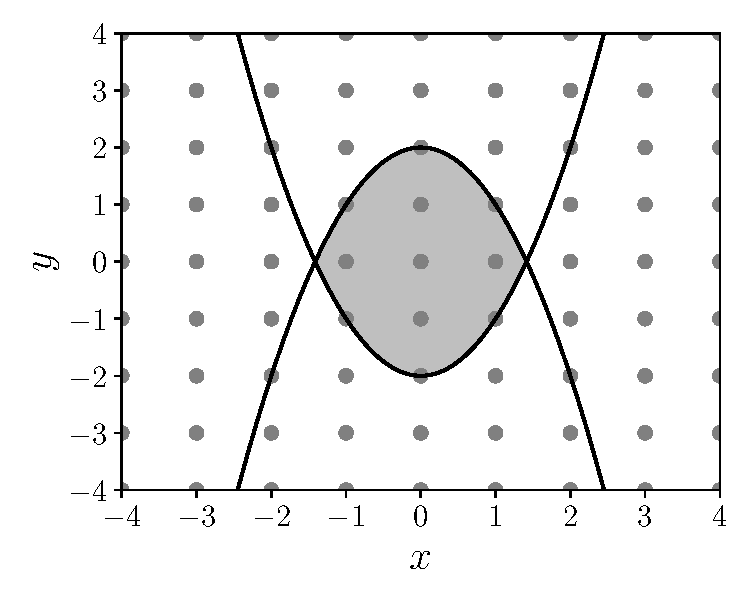
\includegraphics[totalheight=6cm]{chpt5/prob9.pdf}
  			  \caption{A visual representation of the set $C$ for Problems 9 and 10.}
    			   \label{fig:prob_9}
	\end{figure}
\begin{enumerate}

\item 

The joint PMF is:
\[
  P_{XY}(x, y) =
  \begin{cases}
                                   \frac{1}{11} & \text{for $(x, y) \in C$} \\
                                   0 & \text{otherwise} .
  \end{cases}
\]
By looking at Fig.~\ref{fig:prob_9} and adding vertically and horizontally, we can easily determine that the marginal PMFs are:
\[
  P_{X}(x) =
  \begin{cases}
                                   \frac{3}{11} & \text{for $x=-1$} \\
                                   \frac{5}{11} & \text{for $x=0$} \\
                                   \frac{3}{11} & \text{for $x=1$} 
  \end{cases}
\]
and
\[
  P_{Y}(y) =
  \begin{cases}
                                   \frac{1}{11} & \text{for $y=-2$} \\
                                   \frac{3}{11} & \text{for $y=-1$} \\
                                   \frac{3}{11} & \text{for $y=0$} \\
                                   \frac{3}{11} & \text{for $y=1$} \\
                                   \frac{1}{11} & \text{for $y=2$} .
  \end{cases}
\]

\item  Since there are 3 points at $Y=1$, and each point is equally as likely, the total probability mass at $Y=1$ is $3/11$, while the total probability mass at $(-1, 1), (0, 1), (1, 1)$ is 1/11 respectively.  Therefore:
\[
  P_{X|Y}(x|1) =
  \begin{cases}
                                   \frac{1}{3} & \text{for $x=-1$} \\
                                   \frac{1}{3} & \text{for $x=0$} \\
                                   \frac{1}{3} & \text{for $x=1$} .
  \end{cases}
\]

\item $X$ and $Y$ are not independent since, for example, at $X=-1$: $P(X=-1|Y=1) = 1/3 \neq P(X=-1) = 3/11$.

\item Using LOTUS, we have
\begin{equation*}
E[XY^2] = \sum_{(x, y) \in C} xy^2P_{XY}(x, y) = \frac{1}{11}\sum_{(x, y) \in C} xy^2 = \frac{1}{11} \left [1\cdot 1^2+1\cdot(-1)^2 -1\cdot1^2 -1\cdot(-1)^2\right]=0,
\end{equation*}
where only 4 points contribute to the sum (since the rest have zeros).

\end{enumerate}
\end{problem}

\begin{problem}{10} $ $

\begin{enumerate}

\item 

\begin{equation*}
E[X|Y=1] = \sum_{x \in R_{X|Y=1}} x P_{X|Y}(x|1) = (-1)\cdot \frac{1}{3}+(0)\cdot \frac{1}{3}+(1)\cdot \frac{1}{3} =0
\end{equation*}

\item

\begin{equation*}
Var[X|Y=1] = \sum_{x \in R_{X|Y=1}} x^2 P_{X|Y}(x|1) = (1)\cdot \frac{1}{3}+(0)\cdot \frac{1}{3}+(1)\cdot \frac{1}{3} = \frac{2}{3}
\end{equation*}

\item One can easily see that the PMF, $P_{X||Y| \le 1}(x)$ is exactly the same as the PMF for $P_{X|Y}(x|1)$, and therefore the expectation and variance will be the same, thus $E[X||Y| \le 1] =0$.

\item For the same reason as part c of this problem $E[X^2||Y| \le 1] =2/3$.

\end{enumerate}
\end{problem}


\begin{problem}{11} If there are $n$ cars in the shop, then $X = X_1+X_2+ \ldots+ X_n$, where $X_i$ is a $Bern(3/4)$ random variable (as specified in the problem), and where $X_1, X_2, \ldots, X_n$ are all independent (as specified in the problem).  Thus we have that $X|N=n \sim Bin(n, 3/4)$ and for the same reason, $Y|N=n \sim Bin(n, 1/4)$.

\begin{enumerate}

\item Noting that $R_X=R_Y = \{ 0, 1, 2, 3 \}$, we can use the law of total probability to find both of the marginal PMFs, which are:
\begin{align*}
P_X(x) &= \sum_{n=0}^3 P(X=x|N=n)P_N(n) \\
& =  \sum_{n=0}^3 \binom{n}{x} \left( \frac{3}{4} \right)^x \left(\frac{1}{4} \right)^{n-x}P_N(n),
\end{align*}
and 
\begin{align*}
P_Y(y) &= \sum_{n=0}^3 P(Y=y|N=n)P_N(n) \\
& =  \sum_{n=0}^3 \binom{n}{y} \left( \frac{1}{4} \right)^y \left(\frac{3}{4} \right)^{n-y}P_N(n).
\end{align*}
I compute both of these PMFs numerically to find:
\[
  P_{X}(x) \approx
  \begin{cases}
                                   0.180 & \text{for $x=0$} \\
                                   0.258 & \text{for $x=1$} \\
                                  0.352 & \text{for $x=2$} \\
                                  0.211& \text{for $x=3$} \\
                                  0& \text{otherwise},
   \end{cases}
\]
and
\[
  P_{Y}(y) \approx
  \begin{cases}
                                   0.570 & \text{for $y=0$} \\
                                   0.336 & \text{for $y=1$} \\
                                  0.086 & \text{for $y=2$} \\
                                  0.008& \text{for $y=3$} \\
                                  0& \text{otherwise},
   \end{cases}
\]
which, as a sanity, both add up to approximately 1.  We see that since a 4 door car is more likely than a 2 door car, the marginalized PMF for the 4 door cars skews towards high numbers, while the marginalized PMF for the 2 door cars skews towards lower numbers.

\item 

We can find the joint PMF for $X$ and $Y$ by conditioning on $N$ and using the law of total probability:
\begin{equation*}
P_{XY}(x, y) = \sum_{n=0}^3 P(X=x, Y=y|N=n)P_N(n),
\end{equation*}
where we can get rid of the sum because the probability is 0 if $x+y \ne n$:
\begin{align*}
P_{XY}(x, y) &=P(X=x, Y=y|N=x+y)P_N(x+y) \\
& = P(X=x|Y=y, N=x+y) P(Y=y|N=x+y)P_N(x+y) \\
& = P(Y=y|N=x+y)P_N(x+y) \\
& = \binom{x+y}{y}\left (\frac{1}{4} \right)^{y}\left (\frac{3}{4} \right)^{x} P_N(x+y),
\end{align*}
where in the second line I have used the chain rule of probability, in the third I have used the fact that given $Y=y$ and $N=x+y$, we are sure that $X=x$, and in the fourth line I have used the fact that $Y|N=x+y \sim Bin(x+y, 1/4)$.  I compute the joint PMF numerically and present the results in the following table:
\begin{center}
$P_{XY}(x, y) \approx $
\bgroup
\def\arraystretch{2.5}
 \begin{tabular}{ | c | c | c | c | c |}
    \hline
     & $Y=0$ & $Y=1$ & $Y=2$ & $Y=3$ \\  \hline
     $X=0$ &  0.125 &  0.031  &  0.016 &  0.008 \\ \hline
     $X=1$ & 0.094  &  0.094  &  0.070 &  0 \\ \hline
     $X=2$ &  0.141 &  0.211 &  0 &  0 \\ \hline
     $X=3$ & 0.211 &  0 &  0 &  0  \\
    \hline 
  \end{tabular}
  \egroup
\end{center}
As a check, I made sure that the above PMF sums to approximately 1.

\item $X$ and $Y$ are not independent since $P_{XY}(x, y) \ne  P_{X}(x) P_{Y}(y)$ $\forall x, y$.  For example $P_{XY}(0, 0) =0.125$, while $P_{X}(0)P_{Y}(0) \approx 0.180 \cdot 0.570 = 0.103$.

\end{enumerate}

\end{problem}


\begin{problem}{12} I first note that $R_X=R_Y=\{1, 2, 3, 4, 5 \}$ and $R_Z=\{-4, -3, \ldots, 3, 4 \}$.  I can find $P_Z(z)$ by conditioning on either $X$ or $Y$ and by using independence:
\begin{align*}
P_Z(z) &= P(Z = z) \\
& = P(Y=X-z) \\
& = \sum_{x=1}^5 P(Y=X-z|X=x)P_X(x) \\
& = \frac{1}{5}\sum_{x=1}^5 P(Y=x-z|X=x) \\
& = \frac{1}{5}\sum_{x=1}^5 P(Y=x-z) \\
& = \frac{1}{25}\sum_{x=1}^5 \mathbbm{1}\{x-z\in R_Y \},
\end{align*}  
where in going from the fourth to fifth line I used independence.  Thus we have:
\[
  P_{Z}(z) =
  \begin{cases}
                                   \frac{1}{25} & \text{for $z=-4$} \\
                                    \frac{2}{25} & \text{for $z=-3$} \\
                                   \frac{3}{25} & \text{for $z=-2$} \\
                                   \frac{4}{25} & \text{for $z=-1$} \\
                                   \frac{5}{25} & \text{for $z=0$} \\
                                    \frac{4}{25} & \text{for $z=1$} \\
                                     \frac{3}{25} & \text{for $z=2$} \\
                                      \frac{2}{25} & \text{for $z=3$} \\
                                       \frac{1}{25} & \text{for $z=4$}.
   \end{cases}
\]


\end{problem}



\begin{problem}{13} $ $
\begin{enumerate}

\item 

	\begin{equation*}  
  P_X(x) = \begin{cases}
                                   \frac{1}{6}+\frac{1}{6}+\frac{1}{8} & \text{for $x = 0$} \\
                                   \frac{1}{8}+\frac{1}{6}+\frac{1}{4} & \text{for $x = 1$} 
       \end{cases} \quad
= \begin{cases}
                                   \frac{11}{24}& \text{for $x = 0$} \\
                                   \frac{13}{24} & \text{for $x = 1$} 
       \end{cases}
\end{equation*}

	\begin{equation*}  
  P_Y(y) = \begin{cases}
                                   \frac{1}{6}+\frac{1}{8} & \text{for $y = 0$} \\
                                   \frac{1}{6}+\frac{1}{6} & \text{for $y = 1$} \\
                                   \frac{1}{8}+\frac{1}{4} & \text{for $y = 2$} 
       \end{cases} \quad
= \begin{cases}
                                   \frac{7}{24}& \text{for $y = 0$} \\
                                   \frac{1}{3} & \text{for $y = 1$} \\
                                   \frac{3}{8} & \text{for $y = 2$} 
       \end{cases}
\end{equation*}

\item

	\begin{equation*}  
  P_{X|Y}(x|0) = \begin{cases}
                                   \frac{\frac{1}{6}}{\frac{1}{6}+\frac{1}{8}}& \text{for $x = 0$} \\
                                   \frac{\frac{1}{8}}{\frac{1}{6}+\frac{1}{8}}& \text{for $x = 1$} 
       \end{cases} \quad
= \begin{cases}
                                   \frac{4}{7}& \text{for $x = 0$} \\
                                   \frac{3}{7} & \text{for $x = 1$} 
       \end{cases}
\end{equation*}

	\begin{equation*}  
  P_{X|Y}(x|1) = \begin{cases}
                                   \frac{\frac{1}{6}}{\frac{1}{6}+\frac{1}{6}}& \text{for $x = 0$} \\
                                   \frac{\frac{1}{6}}{\frac{1}{6}+\frac{1}{6}}& \text{for $x = 1$} 
       \end{cases} \quad
= \begin{cases}
                                   \frac{1}{2}& \text{for $x = 0$} \\
                                   \frac{1}{2} & \text{for $x = 1$} 
       \end{cases}
\end{equation*}

	\begin{equation*}  
  P_{X|Y}(x|2) = \begin{cases}
                                   \frac{\frac{1}{8}}{\frac{1}{8}+\frac{1}{4}}& \text{for $x = 0$} \\
                                   \frac{\frac{1}{4}}{\frac{1}{8}+\frac{1}{4}}& \text{for $x = 1$} 
       \end{cases} \quad
= \begin{cases}
                                   \frac{1}{3}& \text{for $x = 0$} \\
                                   \frac{2}{3} & \text{for $x = 1$} 
       \end{cases}
\end{equation*}

\item We know that

\[
  Z =
  \begin{cases}
                                   E[X|Y=0]& \text{with probability $P_Y(0)$} \\
                                   E[X|Y=1]& \text{with probability $P_Y(1)$} \\
                                  E[X|Y=2]& \text{with probability $P_Y(2)$},
   \end{cases}
\]
or in other words:
 \[
  P_{Z}(z) =
  \begin{cases}
                                   P_Y(0) & \text{for $z=E[X|Y=0]$} \\
                                    P_Y(1) & \text{for $z=E[X|Y=1]$} \\
                                   P_Y(2) & \text{for $z=E[X|Y=2]$}.
   \end{cases}
\]
We already know the marginal PMF of $Y$, and thus what is left to calculate is $E[X|Y=y]$ for all $y \in R_Y$:
\begin{align*}
E[X|Y=0] &= \sum_{x \in R_X} x P_{X|Y}(x|0) \\
& = 0 \left(\frac{4}{7} \right)+1 \left(\frac{3}{7} \right) \\
& = \frac{3}{7},
\end{align*}
\begin{align*}
E[X|Y=1] &= \sum_{x \in R_X} x P_{X|Y}(x|1) \\
& = 0 \left(\frac{1}{2} \right)+1 \left(\frac{1}{2} \right) \\
& = \frac{1}{2},
\end{align*}
\begin{align*}
E[X|Y=2] &= \sum_{x \in R_X} x P_{X|Y}(x|2) \\
& = 0 \left(\frac{1}{3} \right)+1 \left(\frac{2}{3} \right) \\
& = \frac{2}{3}.
\end{align*}
Finally, we have that:
 \[
  P_{Z}(z) =
  \begin{cases}
                                   \frac{7}{24}& \text{for $z=\frac{3}{7}$} \\
                                    \frac{1}{3} & \text{for $z=\frac{1}{2}$} \\
                                   \frac{3}{8} & \text{for $z=\frac{2}{3}$}.
   \end{cases}
\]


\item For this problem we are checking that the law of iterated expectations holds.  That is, we need to check explicitly that $E[X] = E[E[X|Y]]$, where the outer expectation on the RHS is over $Y$.  Computing the LHS I have:
\begin{equation*}
E[X] = \sum_{x \in R_X} x P_X(x) = 0\left (\frac{11}{24} \right)+1\left (\frac{13}{24} \right) = \frac{13}{24}.
\end{equation*}
Computing the RHS I have:
\begin{align*}
E[Z] &= E_Y[E[X|Y]] \\
& = \sum_{y \in R_Y} E[X|Y=y] P_Y(y) \\
&=\left ( \frac{3}{7} \right ) \left (\frac{7}{24} \right)+\left ( \frac{1}{2} \right ) \left (\frac{1}{3} \right)+\left ( \frac{2}{3} \right ) \left (\frac{3}{8} \right) \\
& = \frac{13}{24}.
\end{align*}
The LHS and RHS agree, and thus the law of iterated expectations holds.

\item 

\begin{align*}
E[Z^2] &= \sum_{z \in R_Z} z^2 P_Z(z) \\
& = \left ( \frac{3}{7} \right )^2 \left (\frac{7}{24} \right)+\left ( \frac{1}{2} \right )^2 \left (\frac{1}{3} \right)+\left ( \frac{2}{3} \right )^2 \left (\frac{3}{8} \right) \\
& =\frac{17}{56}
\end{align*}
$\implies$
\begin{equation*}
Var[Z] = E[Z^2] - E[Z]^2 =  \frac{17}{56} - \left( \frac{13}{24}\right)^2 =\frac{41}{4032}
\end{equation*}

\end{enumerate}
\end{problem}


\begin{problem}{14} $ $
\begin{enumerate}


\item As with the previous problem, we know that

\[
  V =
  \begin{cases}
                                   Var[X|Y=0]& \text{with probability $P_Y(0)$} \\
                                   Var[X|Y=1]& \text{with probability $P_Y(1)$} \\
                                  Var[X|Y=2]& \text{with probability $P_Y(2)$},
   \end{cases}
\]
or in other words:
 \[
  P_{V}(v) =
  \begin{cases}
                                   P_Y(0) & \text{for $v=Var[X|Y=0]$} \\
                                    P_Y(1) & \text{for $v=Var[X|Y=1]$} \\
                                   P_Y(2) & \text{for $v=Var[X|Y=2]$}.
   \end{cases}
\]
Thus, we must compute $Var[X|Y=y] = E[X^2|Y=y]+E[X|Y=y]^2$ for all $y \in R_Y$.  $E[X|Y=y]$ was already computed in the previous problem, and, since to compute $E[X^2|Y=y]$, both terms in the summation are the same as the two terms in the summation to compute $E[X|Y=y]$ (since $0^2=0$ and $1^2=1$), we have that $E[X^2|Y=y]=E[X|Y=y]$ (this can be seen more clearly if one explicitly writes out the summation for $E[X^2|Y=y]$).  Thus we have that:
\begin{equation*}
Var[X|Y=0] =  E[X^2|Y=0]-E[X|Y=0]^2 = \frac{3}{7} -\left ( \frac{3}{7} \right)^2 = \frac{12}{49},
\end{equation*}
\begin{equation*}
Var[X|Y=1] =  E[X^2|Y=1]-E[X|Y=1]^2 = \frac{1}{2} -\left ( \frac{1}{2} \right)^2 = \frac{1}{4},
\end{equation*}
and
\begin{equation*}
Var[X|Y=2] =  E[X^2|Y=2]-E[X|Y=2]^2 = \frac{2}{3} -\left ( \frac{2}{3} \right)^2 = \frac{2}{9}.
\end{equation*}
The PMF for $V$ is thus
 \[
  P_{V}(v) =
  \begin{cases}
                                   \frac{7}{24} & \text{for $v=\frac{12}{49}$} \\
                                    \frac{1}{3} & \text{for $v=\frac{1}{4}$} \\
                                   \frac{3}{8} & \text{for $v=\frac{2}{9}$}.
   \end{cases}
\]

\item
\begin{equation*}
E[V] = \sum_{v \in R_V}v P_V(v) = \frac{12}{49}\cdot \frac{7}{24}+ \frac{1}{4}\cdot \frac{1}{3}+ \frac{2}{9}\cdot \frac{3}{8} =\frac{5}{21}
\end{equation*}

\item In this problem we are checking that the law of total variance, $Var[X] = E_Y[Var[X|Y]]+Var_Y[E[X|Y]]$, holds (where the subscript $Y$ on the expectation and variance denotes with respect to the random variable $Y$.)  Computing the LHS:
\begin{align*}
Var[X] &= E[X^2]-E[X]^2\\
& = \sum_{x \in R_X}x^2 P_X(x)- \left[\sum_{x \in R_X}x P_X(x)\right]^2 \\
& = 0^2\cdot \frac{11}{24}+1^2\cdot \frac{13}{24}-\left[ 0\cdot \frac{11}{24}+1\cdot \frac{13}{24} \right]^2\\
&=\frac{143}{576}.
\end{align*}
Computing the RHS:
\begin{align*}
E_Y[Var[X|Y]]+Var_Y[E[X|Y]] & = E[V]+Var[Z] \\
& = \frac{5}{21}+\frac{41}{4032} \\
& = \frac{143}{576},
\end{align*}
which is in agreement with the LHS of the equation.  Note that $E[V]$ and $Var[Z]$ were computed in this problem and the previous problem.

\end{enumerate}
\end{problem}



\begin{problem}{15} The law of total expectation gives:
\begin{align*}
E[Y] &= \sum_{n=0}^\infty E[Y|N=n]P_N(n) \\
& = \sum_{n=0}^\infty E\left [\sum_{i=1}^N X_i|N=n \right ]P_N(n) \\
& = \sum_{n=0}^\infty E\left [\sum_{i=1}^n X_i \right ]P_N(n) \\
& = \sum_{n=0}^\infty  \sum_{i=1}^n E[X_i] P_N(n) \\
& = \sum_{n=0}^\infty  \sum_{i=1}^n E[X_i] \frac{e^{-\beta} \beta^n}{n!} \\
& = \sum_{n=0}^\infty  \sum_{i=1}^n \frac{1}{\lambda} \frac{e^{-\beta} \beta^n}{n!} \\
& =\frac{e^{-\beta}}{\lambda} \sum_{n=0}^\infty \frac{n \beta^n}{n!},
\end{align*}
where in going from the second to the third line I have used the fact that $X_i$ and $N$ are independent (for all $i$), in going from the third to the fourth line I have used the linearity of expectation, and in going from the fifth to sixth line I have used the fact that for an $Exp(\lambda)$ distribution, $E[X] = 1/\lambda$ .  This summation can be computed by considering the Taylor expansion of the exponential, $\exp(x) = \sum_{n=0}^\infty (x^n)/n!$.  Taking the derivative of both sides of this formula with respect to $x$, we find that the desired sum is:
\begin{equation*}
 \sum_{n=0}^\infty \frac{n x^n}{n!} = xe^x,
\end{equation*}
and hence
\begin{equation*}
E[Y] = \frac{\beta}{\lambda}.
\end{equation*} 
The calculation for $Var[Y]$ is similar.  For this calculation, we will need $\sum_{n=0}^\infty (n^2 x^n)/n!$, which can be found with the same differentiation strategy.  I differentiate the equation for the previous summation with respect to $x$ once more and solve for the desired summation to find
\begin{equation*}
 \sum_{n=0}^\infty \frac{n^2 x^n}{n!} = xe^x+x^2e^x,
\end{equation*}
where I have used the chain rule in differentiating.

To find $Var[Y]$ I now solve for $E[Y^2]$, which is only moderating more complicated than solving for $E[Y]$.  The law of total expectation gives:
\begin{align*}
E[Y^2] &= \sum_{n=0}^\infty E[Y^2|N=n]P_N(n) \\
& = \sum_{n=0}^\infty E\left [\left ( \sum_{i=1}^N X_i \right )^2|N=n \right ]P_N(n) \\
& = \sum_{n=0}^\infty E\left [\left ( \sum_{i=1}^n X_i \right )^2 \right ]P_N(n) \\
& = \sum_{n=0}^\infty E\left [\sum_{i=1}^n X_i^2+ \sum_{j, k: j \neq k} X_j X_k\right ]P_N(n) \\
& = \sum_{n=0}^\infty \left \{\sum_{i=1}^n E[X_i^2]+ \sum_{j, k: j \neq k}  E[X_j X_k] \right \}P_N(n) \\
& = \sum_{n=0}^\infty \left \{\sum_{i=1}^n E[X_i^2]+ \sum_{j, k: j \neq k}  E[X_j] E[X_k] \right \}P_N(n) \\
& = \sum_{n=0}^\infty \left \{\sum_{i=1}^n \frac{2}{\lambda^2}+\sum_{j, k: j \neq k} \frac{1}{\lambda^2} \right \}P_N(n) \\
& = \sum_{n=0}^\infty \left [ \frac{2n}{\lambda^2}+ \frac{n^2-n}{\lambda^2} \right ]\frac{e^{-\beta} \beta^n}{n!} \\
& = \frac{e^{-\beta}}{\lambda^2}\sum_{n=0}^\infty \frac{n \beta^n}{n!}+ \frac{e^{-\beta}}{\lambda^2}\sum_{n=0}^\infty \frac{n^2 \beta^n}{n!},
\end{align*}
where in going from the second to third line I have used the fact that $X_i$ and $N$ are independent (for all $i$), in going from the third to fourth line I have broken the square of the summation into the summation of the squares plus the summation of the cross-terms.  The notation $\sum_{j, k: j \neq k}$ denotes a sum over all possible tuples of $(j,k)$, where $j, k =1, 2, \ldots, n$, except the tuples where $j=k$. In going from the fourth to fifth line I have used the linearity of expectation, in going from the fifth to sixth line I have used the independence of all $X_i$s, and in going from the sixth to seventh line I have used the fact that for an $Exp(\lambda)$ distribution, $E[X^2] = 2/\lambda^2$ (as calculated in the book).  The first summation summation has already been solved for, and to solve the second summation, I use the formula for $\sum_{n=0}^\infty \frac{n^2 x^n}{n!} $ as derived above.  Thus I have that
\begin{align*}
E[Y^2] &= \frac{1}{\lambda} \cdot \frac{\beta}{\lambda}+ \frac{e^{-\beta}}{\lambda^2} \left (\beta e^{\beta}+\beta^2 e^{\beta} \right) \\
& = \frac{\beta^2 +2 \beta}{\lambda^2}.
\end{align*}
Finally we have that:
\begin{align*}
Var[Y] &=  E[Y^2]  -E[Y]^2 \\
&=  \frac{\beta^2 +2 \beta}{\lambda^2} -\frac{\beta^2}{\lambda^2} \\
& = \frac{2 \beta}{\lambda^2}.
\end{align*}

\end{problem}


\begin{problem}{16} $ $
\begin{enumerate}

\item 
\begin{align*}
1 &= \int_0^1 \int_0^\infty f_{XY}(x, y)dx dy \\
& = \int_0^1 \int_0^\infty \frac{1}{2}e^{-x} dx dy+c\int_0^1 \int_0^\infty \frac{y}{(1+x)^2}dx dy \\
& = \int_0^1 \int_0^\infty \frac{1}{2}e^{-x} dx dy+c\int_0^1 \int_1^\infty \frac{y}{u^2}du dy \\
& = \frac{1}{2}+\frac{c}{2}
\end{align*}
$\implies$
\begin{equation*}
c = 1
\end{equation*}


\item 
\begin{align*}
P\left(0 \le X \le 1, 0 \le Y \le \frac{1}{2} \right) &= \int_0^{1/2} \int_0^{1} f_{XY}(x, y)dx dy \\
&= \int_0^{1/2} \int_0^{1} \left [ \frac{1}{2}e^{-x} + \frac{y}{(1+x)^2} \right ]dx dy \\
& = \frac{1}{4}(1-e^{-1})+\frac{1}{16}\\
& \approx 0.22
\end{align*}

\item 
\begin{align*}
P(0 \le X \le 1) &= \int_0^{1} \int_0^{1} f_{XY}(x, y)dx dy \\
&= \int_0^{1} \int_0^{1} \left [ \frac{1}{2}e^{-x} + \frac{y}{(1+x)^2} \right ]dx dy \\
& = \frac{1}{2}(1-e^{-1})+\frac{1}{4}\\
& \approx 0.57
\end{align*}



\end{enumerate}
\end{problem}


\begin{problem}{17} $ $
\begin{enumerate}

\item 

\begin{align*}
f_X(x) &= \int_{R_Y} f_{XY}(x, y)dy \\
&= \int_{0}^\infty e^{-xy}dy \\
&= -\left( \frac{e^{-xy}}{x}\right)_0^\infty \\
& = \frac{1}{x}
\end{align*}
$\implies$
\[
  f_X(x) =
  \begin{cases}
                                   \frac{1}{x}& \text{for $1 \le x< e$} \\
                                   0& \text{otherwise}
   \end{cases}
\]

\begin{align*}
f_Y(y) &= \int_{R_X} f_{XY}(x, y)dx \\
&= \int_{1}^e e^{-xy}dx \\
&= -\left( \frac{e^{-xy}}{y}\right)_1^e \\
& = \frac{1}{y} \left(\frac{1}{e^y}-\frac{1}{e^{ey}} \right)
\end{align*}
$\implies$
\[
  f_Y(y) =
  \begin{cases}
                                    \frac{1}{y} \left(\frac{1}{e^y}-\frac{1}{e^{ey}} \right)& \text{for $y>0$} \\
                                   0& \text{otherwise}
   \end{cases}
\]

\item 

\begin{equation*}
P(0 \le Y \le 1, 1 \le X\le \sqrt{e}) = \int_0^1\int_1^{\sqrt{e}} e^{-xy} dx dy
\end{equation*}



\end{enumerate}
\end{problem}

\begin{problem}{18} $ $
\begin{enumerate}


\item
\begin{align*}
f_X(x) &= \int_{R_Y} f_{XY}(x, y)dy \\
&= \int_{0}^2 \left(\frac{1}{4}x^2+\frac{1}{6}y \right )dy \\
& = \frac{1}{2}x^2+\frac{1}{3}
\end{align*}
$\implies$
\[
  f_X(x) =
  \begin{cases}
                                    \frac{1}{2}x^2+\frac{1}{3}& \text{for $-1 \le x\le 1$} \\
                                   0& \text{otherwise}
   \end{cases}
\]


\begin{align*}
f_Y(y) &= \int_{R_X} f_{XY}(x, y)dx \\
&= \int_{-1}^1 \left(\frac{1}{4}x^2+\frac{1}{6}y \right )dx \\
& = \frac{1}{3}y+\frac{1}{6}
\end{align*}
$\implies$
\[
  f_Y(y) =
  \begin{cases}
                                    \frac{1}{3}y+\frac{1}{6}& \text{for $0 \le y\le 2$} \\
                                   0& \text{otherwise}
   \end{cases}
\]

\item
\begin{align*}
P(X>0, Y<1) &= \int_{0}^1 \int_0^1\left( \frac{1}{4}x^2+\frac{1}{6}y \right)dxdy \\
&= \frac{1}{6}
\end{align*}

\item Using inclusion-exclusion:
\begin{align*}
P(X>0 \cup Y<1) &= P(X>0)+P(Y<1)-P(X>0, Y<1)\\
& = \int_{0}^1 \int_0^2\left( \frac{1}{4}x^2+\frac{1}{6}y \right)dydx +\int_{-1}^1 \int_0^1\left( \frac{1}{4}x^2+\frac{1}{6}y \right)dydx -\frac{1}{6} \\
&\frac{1}{2}+\frac{1}{3} -\frac{1}{6} \\
&= \frac{2}{3}.
\end{align*}

\item
\begin{align*}
P(X>0|Y<1) &= \frac{P(X>0, Y<1)}{P(Y<1)}\\
& = \frac{\frac{1}{6}}{\frac{1}{3}} \\
&= \frac{1}{2}.
\end{align*}

\item
We must be slightly care in choosing the bounds of integration for this problem.  The upper bound of the $y$ integral is the upper bound of $R_Y$, and the lower bound of the $y$ integral is $\max \{0, -x\}$, and not simply $-x$.  This is because for $x>0$, $-x<0$, but the lower bound of the range of $Y$ is 0.  An illustration of the domain of the double integral is shown in Fig.~\ref{fig:prob_18}.  The probability we seek is thus:

\begin{align*}
P(X+Y>0) &= P(Y>-X)\\
& = \int_{-1}^1 \int_{\max \{0, -x\} }^2\left( \frac{1}{4}x^2+\frac{1}{6}y \right)dydx \\
&= \int_{-1}^1 \left [\frac{1}{4}x^2 y +\frac{1}{12}y^2 \right]_{\max \{ 0, -x \} }^2 dx \\
&= \frac{1}{4}\int_{-1}^1 x^2 \left(2-\max \{0, -x\} \right) dx+ \frac{1}{12}\int_{-1}^1 \left(4-\max \{0, -x\}^2 \right) dx \\
&= \frac{1}{4}\int_{-1}^0 x^2 \left(2+x \right) dx+ \frac{1}{4}\int_{0}^1 2 x^2 dx+ \frac{1}{12}\int_{-1}^0 \left(4-x^2 \right) dx+\frac{1}{12}\int_{0}^1 4 dx \\
& = \frac{131}{144}.
\end{align*}

	\begin{figure}[t]
	\centering
      		 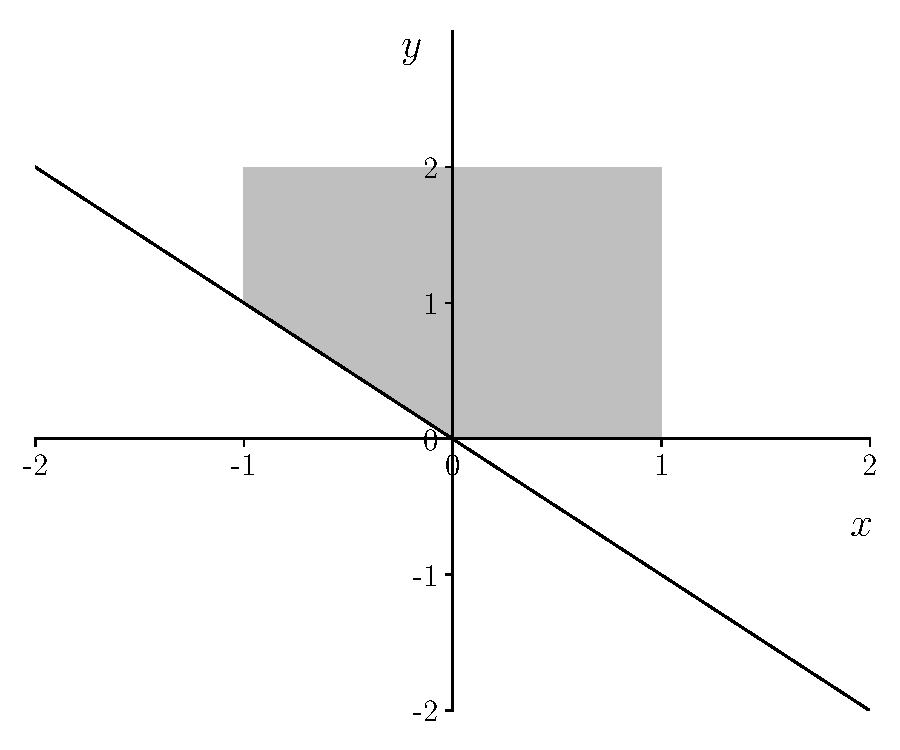
\includegraphics[totalheight=6cm]{chpt5/prob18.pdf}
  			  \caption{The region of integration for Problem 18 (e) (shaded region).}
    			   \label{fig:prob_18}
	\end{figure}

\end{enumerate}
\end{problem}


\begin{problem}{19} $ $
\begin{enumerate}
\item 
\begin{align*}
f_{XY}(x, y) &= \frac{\partial F_{XY}}{\partial x \partial y} \\
& = e^{-x}2e^{-2y}
\end{align*}
$\implies$
\[
  f_{XY}(x, y) =
  \begin{cases}
                                   e^{-x}2e^{-2y}& \text{for $x, y>0$} \\
                                   0& \text{otherwise}
   \end{cases}
\]


\item 
\begin{align*}
P\left(Y>\frac{1}{2}X\right) &= \int_0^\infty \int_0^{x/2}e^{-x}2e^{-2y}dydx \\
& = \int_0^\infty\left(e^{-x}-e^{-2x} \right)dx \\
&=\frac{1}{2}
\end{align*}

\item
$X$ and $Y$ are independent because the joint PDF can be factored into the product of 2 marginal PDFs.  Specifically, the joint PDF can be factored into $f_X(x)f_Y(y)$ where $X\sim Exp(1)$ and where where $Y\sim Exp(2)$.


\end{enumerate}
\end{problem}

\begin{problem}{20} $ $
\begin{enumerate}
\item
To calculate the PDF, we simply need to condition on $X>0$, and since a $\mathcal N(0, 1)$ distribution is symmetric about zero, we know that $P(X>0) =1/2$:
\begin{align*}  
f_{X|X>0}(x) &=\frac{f_X(x)}{P(X>0)} \\
& = \begin{cases}
                                   \frac{2}{\sqrt{2 \pi}} e^{-\frac{x^2}{2}} & \text{for $x >0$} \\
                                   0 & \text{otherwise}.
       \end{cases} \quad
       \end{align*}
To find the conditional CDF, we need only to integrate the Gaussian:
\begin{align*}
F_{X|X>0}(x) &= 2 \int_0^x \frac{1}{\sqrt{2 \pi}}e^{-\frac{{x^\prime}^2}{2}}dx^\prime \\
& =2\left[ \Phi(x) -\frac{1}{2} \right],
\end{align*}
so that
\[
 F_{X|X>0}(x) =
  \begin{cases}
                                   2\Phi(x) -1 & \text{for $x>0$} \\
                                   0& \text{otherwise}.
   \end{cases}
\]

\item
\begin{align*}
E[X|X>0] &= \int_0^\infty x f_{X|X>0}(x)dx \\
& = \frac{2}{\sqrt{2 \pi}} \int_0^\infty x e^{-\frac{x^2}{2}}dx \\
& = \frac{1}{\sqrt{2 \pi}} \int_0^\infty e^{-\frac{u}{2}}du \\
& = \frac{2}{\sqrt{2 \pi}}
\end{align*}


\item We can compute $E[X^2|X>0]$ by noting that if $Y \sim \mathcal N(0, 1)$, then:
\begin{align*}
1 &= E[Y^2] \\
& =\frac{2}{\sqrt{2 \pi} } \int_0^\infty y^2 e^{-\frac{y^2}{2}}dy,
\end{align*}
where I have used the fact that $y^2$ times $\exp{(-y^2/2)}$ is an even function, so I need only integrate from 0 to infinity and multiply by 2.  Thus we have that 
\begin{align*}
E[X^2|X>0] &= \int_0^\infty x^2 f_{X|X>0}(x)dx \\
& = \frac{2}{\sqrt{2 \pi}} \int_0^\infty x^2 e^{-\frac{x^2}{2}}dx \\
& = 1.
\end{align*}
Finally, we have that:
\begin{align*}
Var[X|X>0] &= E[X^2|X>0] -(E[X|X>0] )^2 \\
&=1- \left(\frac{2}{\sqrt{2 \pi}}\right)^2 \\
& =\frac{\pi-2}{\pi}.
\end{align*}

\end{enumerate}

\end{problem}

\begin{problem}{21} $ $
\begin{enumerate}
\item I first find the marginal PDF of $Y$:
\begin{align*}
f_Y(y) &= \int_{-1}^{1} \left(x^2+\frac{1}{3}y\right)dx \\
& =\frac{2}{3}(1+y),
\end{align*}
so that we have
\begin{align*}
f_{X|Y}(x|y) &= \frac{f_{XY}(x,y)}{f_Y(y)} \\
& =\frac{x^2+\frac{1}{3}y}{\frac{2}{3} (1+y)},
\end{align*}
and therefore:
\[
 f_{X|Y}(x|y) =
  \begin{cases}
                                   \frac{3x^2+y}{ 2(1+y)} & \text{for $-1 \le x \le 1$} \\
                                   0& \text{otherwise}.
   \end{cases}
\]



\item 
\begin{align*}
P(X>0|Y=y) &= \int_0^1 f_{X|Y}(x|y)dx \\
&\frac{1}{2(1+y)} \int_0^1 \left(3x^2+y \right) dx \\
& =\frac{1}{2}.
\end{align*}
Notice that the probability, $P(X>0|Y=y)$, does not depend on $y$.

\item We have already found the marginal PDF of $Y$, and now I find the marginal PDF of $X$:
\begin{align*}
f_X(x) &= \int_{0}^{1} \left(x^2+\frac{1}{3}y\right)dy \\
& =x^2 +\frac{1}{6}.
\end{align*}
We thus see that $f_X(x)f_Y(y) = 2x^2/3+y/9+2 y x^2/3+1/9 \ne f_{XY}(x, y)$, and so $X$ and $Y$ are not independent.

\end{enumerate}
\end{problem}


\begin{problem}{22} I start by first finding the marginal PDF of $X$:
\begin{align*}
f_X(x) &= \int_0^1 \left(\frac{1}{2}x^2+\frac{2}{3}y\right)dy \\
& =\frac{1}{2}x^2 +\frac{1}{3},
\end{align*}
which is valid for $-1 \le x \le 1$, otherwise $f_X(x) =0.$

I now find the PDF of $Y$ conditioned on $X=0$:
\begin{align*}
f_{Y|X}(y|0) &= \frac{f_{XY}(0, y)}{f_X(0)} \\
& = \frac{\frac{2}{3}y}{\frac{1}{3}} \\
& = 2y
\end{align*}
valid for $0\le y \le 1$.  I may now calculate $E[Y|X=0],$
\begin{align*}
E[Y|X=0] &= \int_{R_{Y|X=0}} y f_{Y|X}(y|0) dy \\
& = \int_{0}^1 2y^2 dy  \\
& = \frac{2}{3},
\end{align*}
and $E[Y^2|X=0],$
\begin{align*}
E[Y^2|X=0] &= \int_{R_{Y|X=0}} y^2 f_{Y|X}(y|0) dy \\
& = \int_{0}^1 2 y^3 dy  \\
& = \frac{1}{2}.
\end{align*}
Therefore, the variance is: $Var[Y|X=0] = E[Y^2|X=0] - (E[Y|X=0])^2 = 1/2 - (2/3)^2 = 1/18.$

\end{problem}







\begin{problem}{23} $ $
\begin{enumerate}

\item The set $E$ is a diamond shaped region in $\mathbb R^2$, upper-bounded by $1-|x|$ and lower-bounded by $|x|-1$, as shown in Fig.~\ref{fig:prob_23}.  The area of the region is thus 4 times the area of a triangle with a base length of 1 and height length of 1: $4\cdot(1/2)\cdot(1)\cdot(1)=2$.  Since the total probability must integrate to unity, we thus have $c=1/2$.

	\begin{figure}[t]
	\centering
      		 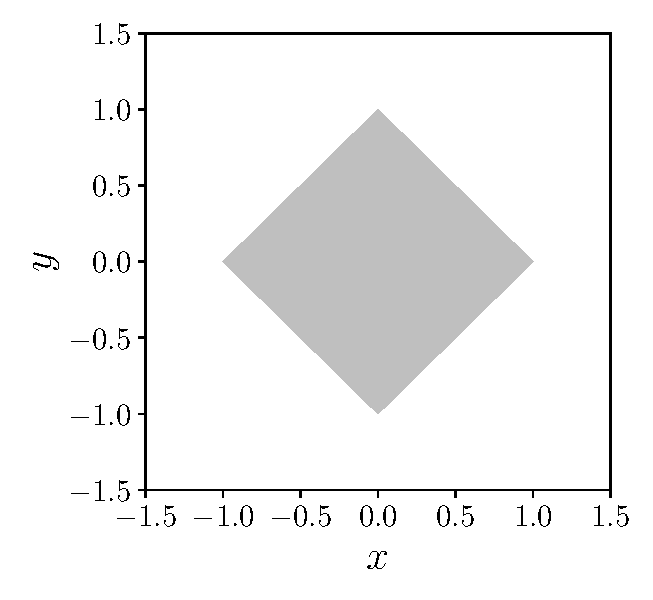
\includegraphics[totalheight=7cm]{chpt5/prob23.pdf}
  			  \caption{A visual representation of the set $E$ for Problem 23.}
    			   \label{fig:prob_23}
	\end{figure}

\item
The marginal PDF of $X$ is given by 
\begin{align*}
f_X(x) &= 2\int_0^{1-|x|} \frac{1}{2} dy \\
& =1-|x|,
\end{align*}
so, that
\[
 f_X(x) =
  \begin{cases}
                                   1-|x| & \text{for $-1 \le x \le 1$} \\
                                   0& \text{otherwise}.
   \end{cases}
\]
By symmetry, we also know that 
\[
 f_Y(y) =
  \begin{cases}
                                   1-|y| & \text{for $-1 \le y \le 1$} \\
                                   0& \text{otherwise}.
   \end{cases}
\]

\item
The conditional PDF is given by
\begin{align*}  
  f_{X|Y}(x|y)&= \frac{f_{XY}(x, y)}{f_Y(y)}\\
& = \begin{cases}
                                   \frac{1}{2(1-|y|)}& \text{for $x, y \in E$} \\
                                   0 & \text{otherwise}.
       \end{cases} \quad
       \end{align*}

\item $X$ and $Y$ are not independent, as it is clear that $f_{X|Y}(x|y) \ne f_X(x)  $.
\end{enumerate}
\end{problem}

\begin{problem}{24}  The marginal PDFs for $X$ and $Y$ are given by 
\[
 f_X(x) =
  \begin{cases}
                                   \frac{1}{2} & \text{for $0 \le x \le 2$} \\
                                   0& \text{otherwise},
   \end{cases}
\]
and
\[
 f_Y(y) =
  \begin{cases}
                                   \frac{1}{2} & \text{for $0 \le y \le 2$} \\
                                   0& \text{otherwise}.
   \end{cases}
\]
I solve for the desired probability by conditioning on $Y$ and using the fact that $X$ and $Y$ are independent:
\begin{align*}
P(XY<1) &= \int_0^2P(XY<1|Y=y)f_Y(y)dy \\
&= \int_0^2P(Xy<1)f_Y(y)dy \\
&= \int_0^2P\left(X<\frac{1}{y}\right)f_Y(y)dy \\
&= \int_0^2 \int_0^{\min \{ 2, 1/y \} }f_X(x) f_Y(y)dxdy \\
&= \frac{1}{4}\int_0^2 \min \left \{ 2, \frac{1}{y} \right \}dy \\
&= \frac{1}{4}\left(\int_0^{1/2}2dy+\int_{1/2}^{2}\frac{1}{y}dy \right)\\
& = \frac{1}{4}+\frac{\ln 2}{2} \\
& \approx 0.60.
\end{align*}

\end{problem}

\begin{problem}{25} The easiest way to solve this problem will be to use the law of iterated expectations and the law of total variance.  The following information will be useful: for $X\sim Exp(1)$, $E[X]=1$, $Var[X]=1$ and $E[X^2]=2$, and for $Y|X \sim Unif(0, X)$, $E[Y|X]=X/2$ and $Var[Y|X] = X^2/12$.
\begin{enumerate}

\item I use the law of iterated expectations, where the subscript on the first expectation denotes an expectation over $X$:
\begin{align*}
E[Y] &= E_X[E[Y|X]] \\
& = E_X\left[\frac{X}{2} \right]\\
& = \frac{1}{2}.
\end{align*}

\item I use the law of total variance, where the subscripts denote expectation and variance over $X$:
\begin{align*}
Var[Y] &= E_X[Var[Y|X]] +Var_X[E[Y|X]]\\
& = E_X\left[\frac{X^2}{12} \right]+Var_X\left[\frac{X}{2} \right]\\\
& = \frac{5}{12}.
\end{align*}

\end{enumerate}
\end{problem}

\begin{problem}{26} For $X \sim Unif(0,1)$ we have: $E[X]=1/2$ and $E[X^2]=1/3$. 
\begin{enumerate}

\item Since $X$ and $Y$ are independent, the expectation of the product is the product of the expectations:
\begin{align*}
E[XY] &= E[X]E[Y] \\
& = \frac{1}{4}.
\end{align*}

\item Since $X$ and $Y$ are independent $E[g(X)h(Y)]=E[g(X)]E[h(Y)]$:
\begin{align*}
E[e^{X+Y}] &= E\left [e^Xe^Y \right] \\
&= E\left [e^X \right ]E\left [e^Y \right]. 
\end{align*}
I can compute $E[e^X]$ using LOTUS:
\begin{align*}
E\left[e^{X}\right] &= \int_0^1 e^x dx \\
& = e-1,
\end{align*}
and plugging into the previous equation I find that
\begin{equation*}
E\left[e^{X+Y}\right] = (e-1)^2.
\end{equation*}

\item 
\begin{align*}
E[X^2+Y^2+XY] &= E[X^2]+E[Y^2]+E[XY] \\
& = \frac{1}{3}+\frac{1}{3}+\frac{1}{4} \\
& = \frac{11}{12}
\end{align*}

\item We can compute this expectation with a 2D LOTUS over the joint distribution of $X$ and $Y$.  Since $X$ and $Y$ are independent, $f_{XY}(x,y) = f_X(x)f_Y(y) = 1$ for $x, y \in [0, 1]$:
\begin{align*}
E[Ye^{XY}] &= \int_0^1 \int_0^1 y e^{xy} dxdy \\
&= \int_0^1 \left (1-e^y \right) dy \\
&= e-2.
\end{align*}

\end{enumerate}
\end{problem}

\begin{problem}{27} I first note that $R_X=R_Y=[0, 1]$ and that $R_Z=[0, \infty)$.  I solve for the CDF of $Z$ by conditioning on $X$ and using the fact that $X$ and $Y$ are independent:
\begin{align*}
F_Z(z) &= P(Z \le z) \\
& = P\left(\frac{X}{Y} \le z\right) \\
& = P\left(Y \ge \frac{X}{z}\right) \\
& = \int_{-\infty}^\infty P \left(Y \ge \frac{x}{z} |X=x\right)f_X(x)dx \\
& = \int_{0}^1 P\left(Y \ge \frac{x}{z}|X=x\right)dx \\
& = \int_{0}^1 P\left(Y \ge \frac{x}{z}\right)dx,
\end{align*}
where in the last line I have used the fact that $X$ and $Y$ are independent.  To solve for $P(Y \ge X/z)$ by integrating $F_Y(y)$ over $y$, some care must be taken in the limits of integration.  Since $x \in [0, 1]$ and $z \in [0, \infty)$, this implies that $x/z \in [0, \infty)$.  However, we know that $f_Y(y) = 0$ for $y>1$ and thus the lower bound of integration is not simply $x/z$, but is $\min \{1, x/z \}$.  This can be seen pictorially in Fig.~\ref{fig:prob_27} a) (from a point of view of integrating over the joint PDF to solve the problem, rather than the conditional PDF), which is the $x-y$ plane, where the grey region corresponds to the region of non-zero joint probability density.  For any given $z$, $P(Y \ge X/z)$ represents the total probability mass above the the line defined by $x/z$.  For example, I have, I have drawn 3 different lines in \ref{fig:prob_27} a) corresponding to $z=1/2$ (highest line), $z=1$ (middle line) and $z=2$ (lowest line).  For each of these $z$ values, $P(Y \ge X/z)$ is the fraction of the grey box above that line.  We see that when $z$ increases from $0$ to $1$ (corresponding to the vertical  line along the $y$-axis and the line $y=x$), the total probability mass above the line increases smoothly.  However, due to the edge of the box, there is a kink in the total probability mass above the line when transitioning from $z<1$ to $z>1$, which is the same reason we will get a kink in the function $F_Z(z)$ due to $\min \{1, x/z \}$.  

	\begin{figure}[t]
	\centering
      		 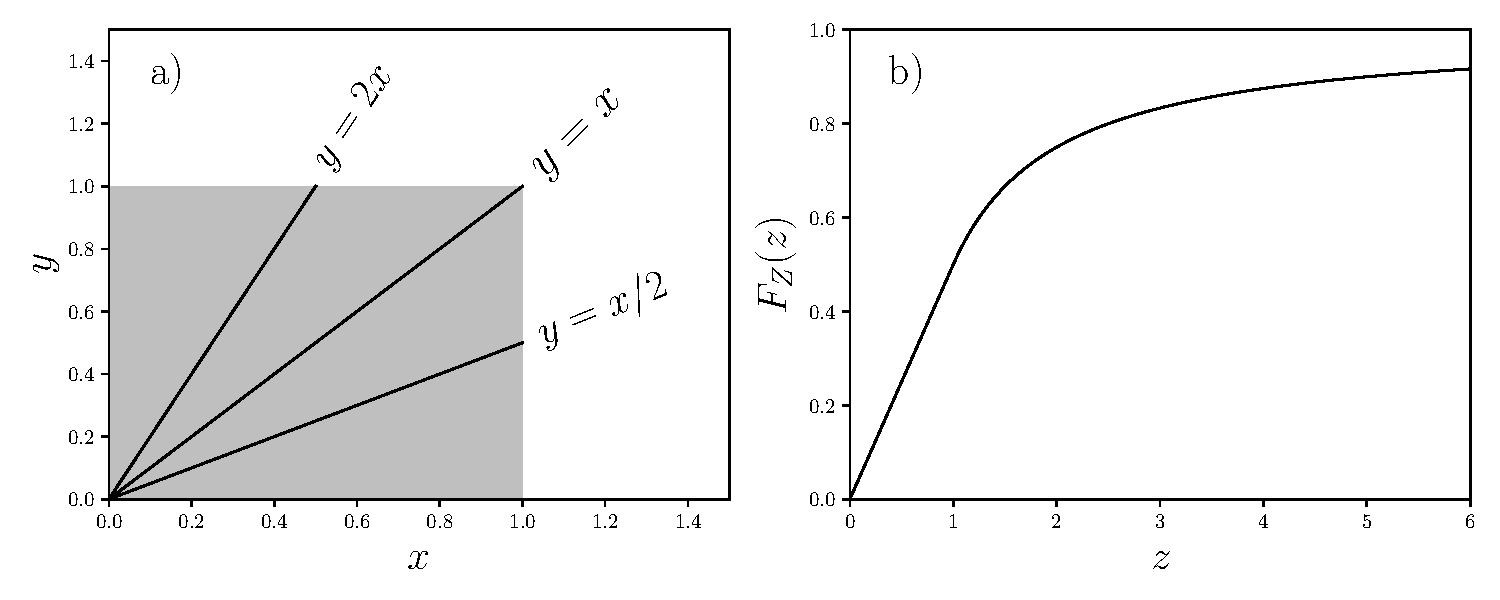
\includegraphics[totalheight=6cm]{chpt5/prob27.pdf}
  			  \caption{a) The $x-y$ plane where the shaded region denotes the region of non-zero probability for the PDF at hand.  b) A plot of the CDF of $Z$.}
    			   \label{fig:prob_27}
	\end{figure}
	
Continuing with the calculation:
\begin{align*}
F_Z(z) &=  \int_{0}^1 P\left(Y \ge \frac{x}{z}\right)dx,\\
& = \int_{0}^1 \int_{\min \{1, x/z \}}^1 f_Y(y)dy dx,\\
& = \int_0^1 \left [1- \min \left \{ 1, \frac{x}{z}\right \} \right]dx \\
& =1 - \int_0^1  \min \left \{ 1, \frac{x}{z}\right \} dx \\
& =1 - \left (\int_0^1 \mathbbm{1} \{x \ge z \}dx+\int_0^1\frac{x}{z} \mathbbm{1} \{x < z \}dx  \right),
\end{align*}
where I have picked out the proper value of the $\min$ function by utilizing an indicator function (which is much nicer to use in an integral since it ``kills" the integral whenever the logical condition evaluates to false).

Thus, for $z>1$ we have that:
\begin{align*}
F_Z(z) &=1 - \int_0^1 \frac{x}{z}dx \\
& =1-\frac{1}{2z},
\end{align*}
while for $z\in [0,1]$ we have that:
\begin{align*}
F_Z(z) &=1 - \left( \int_0^z \frac{x}{z}dx+\int_z^1 dx \right) \\
& =\frac{z}{2}.
\end{align*}
In summary we have:
\[
 F_Z(z) =
  \begin{cases}
                                  \frac{z}{2}& \text{for $0 \le z \le 1$} \\
                                   1 - \frac{1}{2z} & \text {for $z >1$} \\
                                   0& \text {otherwise},
   \end{cases}
\]
which I plot in Fig.~\ref{fig:prob_27} b).  Notice that even though this is a piecewise function, it appears very smooth because, at the transition ($z =1$), both the actual function and the first derivative match between the two piecewise regions.

To find the PDF we need only to differentiate:
\begin{align*}  
f_Z(z) &= \frac{dF_Z(z)}{dz} \\
& = \begin{cases}
                                  \frac{1}{2} &  \text{for $0 \le z \le 1$}\\
                                 \frac{1}{2z^2} &\text {for $z >1$} \\
                                 0& \text {otherwise}.
    \end{cases} \quad
\end{align*}


\end{problem}


\begin{problem}{28} $ $
\begin{enumerate}

\item  To find $f_{U|X}(x|u)$ I first solve for the conditional CDF then differentiate with respect to $u$:
\begin{align*}
F_{U|X}(u|x) &= P(U \le u |X=x) \\
& = P(X+Y \le u |X=x) \\
& = P(x+Y \le u |X=x) \\
& = P(Y \le u -x) \\
& = \Phi(u-x),
\end{align*}
where in the fourth line I have used the fact that $X$ and $Y$ are independent.  To find the conditional PDF I now differentiate:
\begin{align*}
\frac{\partial F_{U|X}}{\partial u} &=  \Phi^\prime(u-x) \\
 &=  \frac{1}{\sqrt{2 \pi}} e^{-\frac{(u-x)^2}{2}},
 \end{align*}
 and thus we see that:
 \begin{equation*}
 U|X=x \sim \mathcal N(x, 1).
 \end{equation*}
 
 \item If $X~\sim \mathcal N (\mu_x, \sigma_x^2)$ and $X~\sim \mathcal N (\mu_y, \sigma_y^2)$ are independent, then, as shown in the book by the method of convolution, $X+Y~\sim \mathcal N (\mu_x+\mu_y, \sigma_x^2+\sigma_y^2)$, and thus:
 \begin{equation*}
 U ~\sim \mathcal N(0, 2).
 \end{equation*}
 
 \item To find $f_{X|U}(x|u)$, I use Baye's rule for PDFs:
 \begin{align*}
f_{X|U}(x|u) & =\frac{f_{U|X}(u|x) f_X(x)}{f_U(u)}\\
& = \frac{\frac{1}{\sqrt{2\pi}} e^{-\frac{(u-x)^2}{2}} \frac{1}{\sqrt{2 \pi}} e^{-\frac{x^2}{2}} }{\frac{1}{2\sqrt{\pi}} e^{-\frac{u^2}{4}}} \\
& =\frac{1}{\sqrt{\pi}}e^{-\frac{(u-x)^2}{2} -\frac{x^2}{2}+\frac{u^2}{4}} \\
&=\frac{1}{\sqrt{\pi}} e^{-\left(x-\frac{u}{2}\right)^2} \\
&=\frac{1}{\sqrt{2 \pi} (1/\sqrt{2})} e^{-\frac{\left(x-\frac{u}{2}\right)^2}{2 \cdot \frac{1}{2}}},
 \end{align*}
 where I have used the ``completing the square" trick in the exponential to make it more Gaussian.  We recognize this distribution as a normal, $u/2$, $1/2$ distribution:
  \begin{equation*}
 X|U=u \sim \mathcal N\left (\frac{u}{2}, \frac{1}{2} \right).
 \end{equation*}

\item Since  $X|U=u \sim \mathcal N\left (\frac{u}{2}, \frac{1}{2} \right)$, we have:
\begin{equation*}
E[X|U=u] =\frac{u}{2},
\end{equation*}
and
\begin{equation*}
Var[X|U=u] =\frac{1}{2}.
\end{equation*}

\end{enumerate}
\end{problem}

\begin{problem}{29} This problem can be solved using the method of transformations.  Since $X$ and $Y$ are independent, we have an axis-aligned 2D Gaussian for the joint distribution:
\begin{align*}
f_{XY}(x,y) &= f_X(x)f_Y(y) \\
& = \frac{1}{ 2 \pi} e^{-\frac{1}{2}(x^2+y^2)}.
\end{align*}
I define the functions $h_1$ and $h_2$ as:
\[
\begin{cases}
               X = h_1(R, \Theta)= R\cos \Theta \\
	       Y = h_2(R, \Theta) = R\sin \Theta,
            \end{cases}
\]
so that, according to the method of transformations:
\begin{equation*}
f_{R\Theta}(r, \theta) = f_{XY}(h_1(r, \theta), h_2(r, \theta)) \begin{vmatrix}
\frac{\partial h_1}{\partial r} & \frac{\partial h_1}{\partial \theta}  \\ 
\frac{\partial h_2}{\partial r} & \frac{\partial h_2}{\partial \theta}
\end{vmatrix}.
\end{equation*}

The Jacobian is easy to calculate:
\begin{align*}
J &=  \begin{vmatrix}
\cos \theta & -r \sin \theta \\ 
\sin \theta & r\cos \theta 
\end{vmatrix}\\
& = r(\cos^2 \theta +\sin^2 \theta ) \\
& = r,
\end{align*}
where I have used the Pythagorean trigonometric identity.  Thus, we have that:
\begin{align*}
f_{R\Theta}(r, \theta) &= \frac{1}{2 \pi} e^{-\frac{(r \cos \theta)^2}{2}}e^{-\frac{(r \sin \theta)^2}{2}} r \\
&= \frac{r}{2 \pi} e^{-\frac{1}{2}r^2},
\end{align*}
where I have again used the Pythagorean trigonometric identity.

If $R$ and $\Theta$ are independent, then we can factor $f_{R\Theta}(r, \theta)$ into $f_{R}(r)f_\Theta(\theta)$.  To help determine what these 2 functions are, I integrate the joint distribution:
\begin{align*}
1 &=\int_0^\infty \int_{-\pi}^\pi f_{R\Theta}(r, \theta) dr d \theta \\
& =\int_0^\infty \int_{-\pi}^\pi \frac{r}{2 \pi} e^{-\frac{1}{2}r^2}dr d \theta \\
& = \int_0^\infty r e^{-\frac{1}{2}r^2}dr.
\end{align*}
Thus, we see that the function $r e^{-\frac{1}{2}r^2}$, which only depends on $r$, is always positive (for $r \ge 0$) and integrates to 1.  This is the marginal distribution of $R$.  The function $1/(2 \pi)$ is always positive and integrates to 1 for $\theta \in [-\pi, \pi]$, and this is thus the marginal distribution of $\Theta$.  Therefore we see that $f_{R\Theta}(r, \theta)$ can be factored into $f_{R}(r)f_\Theta(\theta)$, and thus $R$ and $\Theta$ are independent.



\end{problem}

\begin{problem}{30} If $X, Y\distas{iid} Unif(0, 1)$, then:
\[
 F_{XY}(x,y) =
  \begin{cases}
                                  1 & \text{for $x, y \in [0, 1]$} \\
                                   0 & \text {otherwise}.
   \end{cases}
\]
	\begin{figure}[t]
	\centering
      		 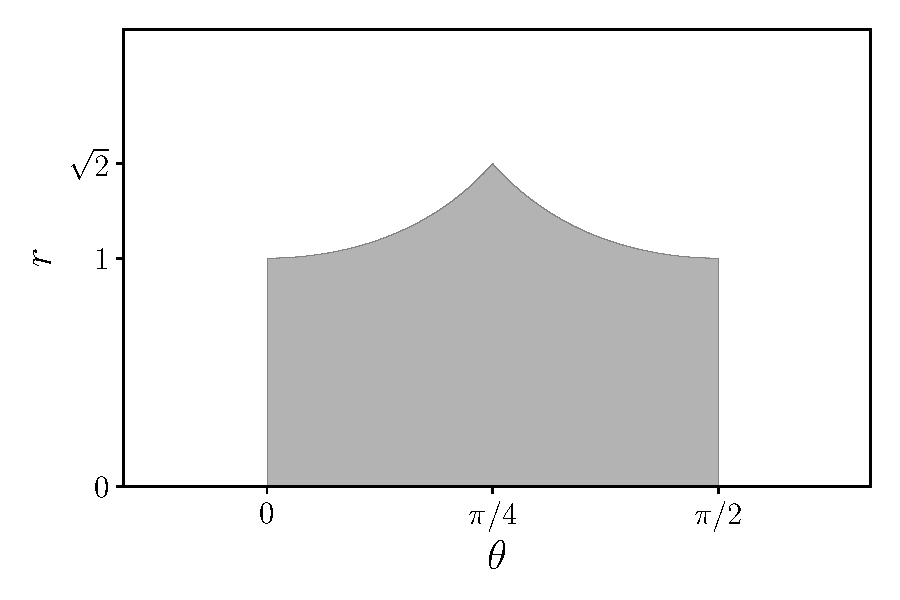
\includegraphics[totalheight=6cm]{chpt5/prob30b.pdf}
  			  \caption{The $r-\theta$ plane for Problem 30.  The grey region denotes the region in the plane where $f_{R\Theta}(r, \theta)$ is non-zero.}
    			   \label{fig:prob_30b}
	\end{figure}
The Jacobian has already been calculated in the previous problem ($J=r$), so that
\begin{align*}  
f_{R\Theta}(r, \theta) &= rF_{XY}(r\cos \theta ,r \sin \theta) \\
& = \begin{cases}
                                  r & \text{for $r\cos \theta ,r \sin \theta \in [0, 1]$} \\
                                   0 & \text {otherwise},
    \end{cases} \quad
\end{align*}
where in Fig.~\ref{fig:prob_30b}, I have indicated where in the $r-\theta$ plane $f_{R\Theta}(r, \theta)$ is non-zero.



We can further examine the constraints $r\cos \theta ,r \sin \theta \in [0, 1]$ to gain more insight.  Satisfying these conditions is equivalent to simultaneously satisfying the following four conditions:
\[
\begin{cases}
               r \cos \theta \le 1\\
               r \sin \theta \le 1\\
               r \cos \theta \ge 0\\
               r \sin \theta \ge 0.
            \end{cases}
\]
Since $r$ is always positive, the last 2 conditions yield $\cos \theta \ge 0 $ and $\sin \theta \ge 0$, which only happens in the first quadrant, i.e., $0 \le \theta \le \pi/2$.  If we plot the first 2 conditions for $0 \le \theta \le \pi/2$, as in Fig.~\ref{fig:prob_30}, we see that when $0 \le \theta \le \pi/4$, $r \cos \theta \le 1 \implies r \sin \theta \le 1$ and when $\pi/4 \le \theta \le \pi/2$, $r \sin \theta \le 1 \implies r \cos \theta \le 1$.

	\begin{figure}[t]
	\centering
      		 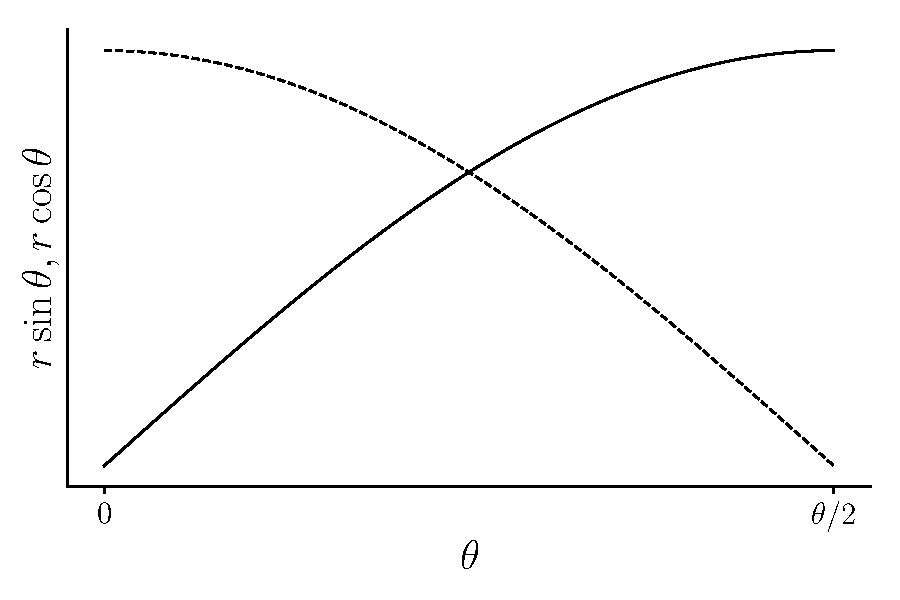
\includegraphics[totalheight=6cm]{chpt5/prob30.pdf}
  			  \caption{$r \sin \theta$ (solid line) and $r \cos \theta$ (dashed line) for $0 \le \theta \le \pi/2$}
    			   \label{fig:prob_30}
	\end{figure}
	
Thus, we can re-write $f_{R\Theta}(r, \theta)$ with the constraints specified a little more explicitly:
\[
 f_{R\Theta}(r, \theta) =
  \begin{cases}
                                  r & \text{for $0 \le \theta \le \frac{\pi}{4}$ and $r \le \frac{1}{\cos \theta}$}  \\
                                   r & \text{for $ \frac{\pi}{4} \le \theta \le \frac{\pi}{2}$ and $r \le \frac{1}{\sin \theta}$}  \\
                                    0 & \text {otherwise},
   \end{cases}
\]
(where the inequalities did not flip when I divided by $\cos \theta$ and $\sin \theta$ because these are both positive in the first quadrant). Note that these constraints imply that $f_{R\Theta}(r, \theta) >0 $ in the unit square and $f_{R\Theta}(r, \theta) =0 $ outside of the unit square, as we would expect for $X, Y \sim Unif(0,1)$ as shown in Fig.~\ref{fig:prob_30c}.  The figure shows the unit square in the $x-y$ plane (where the probability is non-zero), and it shows that for $\theta$ less than $\pi/4$, $r$ is constrained by $0\le r \le 1/ \cos \theta$ (for values of $r$ within the unit square).  One can similarly show in this figure that for $\theta $ greater than $\pi/4$, $0\le r \le 1/ \sin \theta$.

We can check explicitly that this PDF integrates to 1:
\begin{align*}
\int_0^{\frac{\pi}{4}} \int_0^{\frac{1}{\cos \theta}} r dr d\theta+\int_{\frac{\pi}{4}}^{\frac{\pi}{2}} \int_0^{\frac{1}{\sin \theta}} r dr d\theta &= \frac{1}{2}\int_0^{\frac{\pi}{4}}  \frac{1}{\cos^2 \theta}d\theta+\frac{1}{2}\int_{\frac{\pi}{4}}^{\frac{\pi}{2}}\frac{1}{\sin^2 \theta}d\theta \\
&=\frac{1}{2} \tan{\theta}\Big|_0^{\frac{\pi}{4}} -\frac{1}{2} \left(\frac{\cos \theta}{\sin \theta}\right )_{{\frac{\pi}{4}}}^{\frac{\pi}{2}} \\
&=1.
\end{align*}
For this problem $R$ and $\Theta$ are not independent, because there is no way to factor $f_{R\Theta}(r, \theta)$ into an equation of just $r$ times an equation of just $\theta$, since the values of $r$ over which the PDF is non-zero explicitly depend on the values of $\theta$.

	\begin{figure}[t]
	\centering
      		 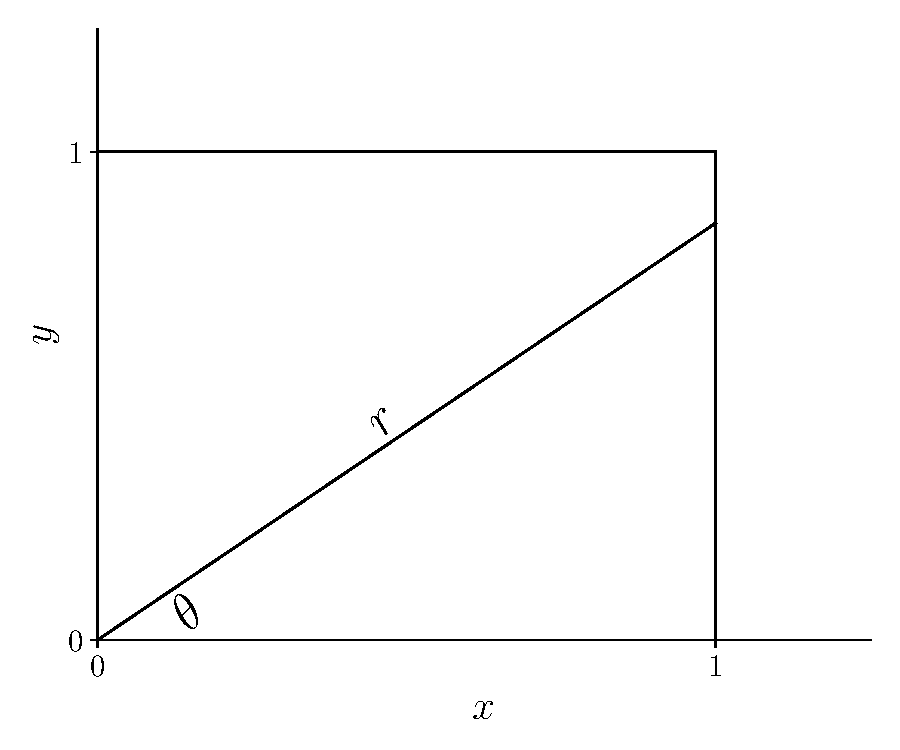
\includegraphics[totalheight=6cm]{chpt5/prob30c.pdf}
  			  \caption{The unit square in the $x-y$ plane.  In polar coordinates, to be within the unit square, it can be seen geometrically that $r$ is constrained by $0\le r \le 1/ \cos \theta$ for $0 \le \theta \le \pi/4$, and by $0\le r \le 1/ \sin \theta$ for $\pi/4< \theta \le \pi/2$.}
    			   \label{fig:prob_30c}
	\end{figure}

\end{problem}

\begin{problem}{31} The covariance can be computed straight from its definition:
\begin{align*}
Cov[X, Y] &= E[XY] -E[X]E[Y] \\
&= \sum_{x=0}^1 \sum_{y=0}^2 xy P_{XY}(x, y)-\left(\sum_{x=0}^1x P_X(x) \right) \left(  \sum_{y=0}^2y P_Y(y) \right) \\
& = 1\cdot \frac{1}{6}+2\cdot \frac{1}{6} -\left[1\cdot \left(\frac{1}{8}+\frac{1}{6}+\frac{1}{6}\right)\right]\left[1\cdot \left(\frac{1}{4}+\frac{1}{6}\right)+2\cdot \left(\frac{1}{8}+\frac{1}{6}\right) \right] \\
& = \frac{1}{24}.
\end{align*}

To calculate $\rho_{XY}$, I first calculate the variances.  For $X$ we have
\begin{equation*}
E[X] = \sum_{x=0}^1xP_X(x) = 1 \cdot \left (\frac{1}{8}+\frac{1}{6}+\frac{1}{6}\right) = \frac{11}{24},
\end{equation*}
\begin{equation*}
E[X^2] = \sum_{x=0}^1x^2P_X(x) = 1 \cdot \left (\frac{1}{8}+\frac{1}{6}+\frac{1}{6}\right) = \frac{11}{24} 
\end{equation*}
$\implies$
\begin{align*}
Var[X] &=E[X^2]-E[X]^2 \\
&=\frac{11}{24}- \left(\frac{11}{24} \right)^2 \\
&=\frac{143}{576},
\end{align*}
and for $Y$ we have
\begin{equation*}
E[Y] = \sum_{y=0}^2yP_Y(y) = 1 \cdot \left  (\frac{1}{4}+\frac{1}{6}\right)+2 \cdot \left (\frac{1}{8}+\frac{1}{6}\right) = 1,
\end{equation*}
\begin{equation*}
E[Y^2] = \sum_{y=0}^2y^2P_Y(y) = 1 \cdot \left (\frac{1}{4}+\frac{1}{6} \right)+2^2 \cdot \left (\frac{1}{8}+\frac{1}{6}\right) = \frac{19}{12}
\end{equation*}
$\implies$
\begin{align*}
Var[Y] &=E[Y^2]-E[Y]^2 \\
&=\frac{19}{12}- 1^2 \\
&=\frac{7}{12}.
\end{align*}
Finally, the correlation is:
\begin{equation}
\rho_{XY} = \frac{Cov[X, Y] }{\sqrt{Var[X] Var[Y]}} = \frac{\frac{1}{24}}{\sqrt{\frac{143}{576} \cdot \frac{7}{12}}} \approx 0.11.
\end{equation}
Thus, there is a weak, positive correlation between $X$ and $Y$.

\end{problem}

\begin{problem}{32} We can use several of the items in Lemma 5.3 in the book to solve this problem:
\begin{align*}
Cov[Z, W] &= Cov[11-X+X^2Y, 3-Y] \\
& = Cov[-X+X^2Y, -Y] \\
& = Cov[X, Y]-Cov[X^2Y, Y] \\
&=-Cov[X^2Y, Y] \\
& = -\left (E[X^2Y^2] -E[X^2Y]E[Y] \right ) \\
& = -\left (E[X^2]E[Y^2] -E[X^2]E[Y]^2 \right ) \\
& =-(1-0) \\
&=-1,
\end{align*}
where in the second line I have used item 5 of Lemma 5.3, in the third item 7, in the fourth item 2 in the sixth I have used the fact that $X$ and $Y$ are independent and in the seventh I have used the fact that $X, Y \sim \mathcal N(0,1)$.
\end{problem}

\begin{problem}{33} To solve this problem I use several of the items in Lemma 5.3 in the book.  Since $Z$ and $W$ are independent, we have that:
\begin{align*}
0 &= Cov[Z, W] \\
& = Cov[2X-Y, X+Y] \\
& = 2Cov[X, X]+2Cov[X, Y]-Cov[Y, X]-Cov[Y, Y] \\
& = 2 Var[X] +Cov[X, Y]-Var[Y] \\
& = 2 \cdot 4+ Cov[X, Y]- 9
\end{align*}
$\implies$
\begin{equation*}
Cov[X, Y] = 1.
\end{equation*}

The correlation is now straightforward to calculate: 
\begin{equation*}
\rho_{XY} = \frac{Cov[X, Y]}{\sqrt{Var[X] Var[Y]}} = \frac{1}{\sqrt{4 \cdot 9}} =\frac{1}{6}.
\end{equation*}


\end{problem}


\begin{problem}{34}
We know that $X \sim Unif(1, 3)$ (so that $E[X] = 2$) and $Y|X=x \sim Exp(x)$ (so that $E[Y|X] = 1/x$).  Since $Cov[X, Y] = E[XY]-E[X]E[Y]$, and since we know the distribution of $Y|X=x$ we can probably solve most of the expectations by conditioning on $X$ and using the law of iterated expectations.  To solve for $E[Y]$ I use the law of iterated expectations (where the subscript $X$ denotes an expectation over the random variable $X$):
\begin{align*}
E[Y] &= E_X[E[Y|X]] \\
 &= E_X\left [\frac{1}{X} \right ]\\
 &= \frac{1}{2}\int_1^3\frac{1}{x}dx \\
 & = \frac{1}{2} \ln 3.
\end{align*}
To solve for $E[XY]$ I also condition on $X$ and ``take out what is known":
\begin{align*}
E[XY] &= E_X[E[XY|X]] \\
 &= E_X[XE[Y|X]] \\
 &= E_X\left [X\frac{1}{X} \right] \\
 & = 1.
\end{align*}
Thus, we have that the covariance is:
\begin{align*}
Cov[X, Y] &= E[XY]-E[X]E[Y] \\
& = 1-2\cdot\frac{1}{2} \ln 3 \\
&= 1- \ln 3.
\end{align*}

\end{problem}

\begin{problem}{35} The covariance is:
\begin{align*}
Cov[Z, W] &= Cov[7+X+Y, 1+Y]\\
& = Cov[X+Y, Y]\\
& = Cov[X,Y]+Var[Y]\\
&= 0+1\\
&=1,
\end{align*}
where I have used the fact that $Cov[X,Y]=0$ since $X$ and $Y$ are independent. Calculating the variances is easy as well:
\begin{equation*}
Var[Z] = Var[7+X+Y] = Var[X]+Var[Y] = 2,
\end{equation*}
and
\begin{equation*}
Var[W] = Var[1+Y] = Var[Y] = 1.
\end{equation*}
Thus we have that the correlation is:
\begin{equation*}
\rho_{ZW} = \frac{Cov[Z, W]}{\sqrt{Var[Z] Var[W] }} = \frac{1}{\sqrt{2}} \approx 0.71.
\end{equation*}

\end{problem}

\begin{problem}{36} $ $
\begin{enumerate}
\item 
\begin{equation*}
X+2Y  \sim \mathcal N(\mu_X+2\mu_Y, \sigma_X^2+4\sigma_Y^2+2 \cdot 2 \rho \sigma_X \sigma_Y) =\mathcal N (1, 4)
\end{equation*}
$\implies$
\begin{equation*}
P(X+2Y \le 3) = \Phi \left (\frac{3-1}{2} \right)= \Phi (1) \approx 0.84.
\end{equation*}

\item

\begin{align*}
Cov[X-Y, X+2Y] & = Cov[X, X]+2 Cov[X, Y]-Cov[X, Y]-2 Cov[Y, Y] \\
& = \sigma_X^2+ \rho \sigma_X \sigma_Y -2 \sigma_Y^2 \\
& = 1
\end{align*}

\end{enumerate}
\end{problem}

\begin{problem}{37} $ $
\begin{enumerate}
\item 
\begin{equation*}
X+2Y  \sim \mathcal N(\mu_X+2\mu_Y, \sigma_X^2+4\sigma_Y^2+2 \cdot 2 \rho \sigma_X \sigma_Y) =\mathcal N (3, 8)
\end{equation*}
$\implies$
\begin{align*}
P(X+2Y > 4) &= 1-P(X+2Y \le 4) \\
& = 1 - \Phi \left (\frac{4-3}{\sqrt{8}} \right) \\
& = 1 - \Phi \left (\frac{1}{2\sqrt{2}} \right) \\
& \approx 0.36.
\end{align*}

\item Since $X$ and $Y$ are uncorrelated, jointly normal random variables they are independent, and thus:
\begin{align*}
E[X^2Y^2] &= E[X^2] E[Y^2] \\
&=(Var[X]+E[X]^2)(Var[Y]+E[Y]^2) \\
&=(\sigma_X^2+\mu_X^2)(\sigma_Y^2+\mu_Y^2) \\
&=10.
\end{align*}

\end{enumerate}
\end{problem}



\begin{problem}{38} $ $
\begin{enumerate}

\item $X$ and $Y$ are jointly normal random variables, and thus by Theorem 5.4 in the book:
\begin{align*}
Y|X=x &\sim \mathcal N \left (\mu_Y+\rho \sigma_Y \frac{x-\mu_X}{\sigma_X}, (1-\rho^2) \sigma_Y^2 \right) \\
&=\mathcal N \left(1-\frac{3(x-2)}{4}, \frac{27}{4} \right).
\end{align*}
We therefore can immediately read off that 
\begin{equation*}
E[Y|X=3] =1 -\frac{3(3-2)}{4} = \frac{1}{4}.
\end{equation*}

\item Using the same distribution:
\begin{equation*}
Var[Y|X=2] =\frac{27}{4}.
\end{equation*}

\item To solve for this problem, I define the random variables $U = X+2Y$ and $V=X+Y$ and I solve for the distribution of $U|V$.  Since $X$ and $Y$ are jointly normal random variables, so too are $U$ and $V$ (since $aU+bV = aX+2aY+bX+bY=(a+b)\cdot X+(2a+b)\cdot Y$ which we know is normal for all $a, b$) and thus Theorem 5.4 in the book gives an equation for the distribution of $U|V$.  But first to use this formula, we will need to explicitly compute the distributions of $U$ and $V$.  The distribution of $U$ is 
\begin{align*}
U &\sim \mathcal N(\mu_X+2\mu_Y, \sigma_X^2+4 \sigma_Y^2+2\cdot2\rho \sigma_X \sigma_Y) \\
& = \mathcal N(4, 28),
\end{align*}
and the distribution of $V$ is
\begin{align*}
V & \sim \mathcal N(\mu_X+\mu_Y, \sigma_X^2+\sigma_Y^2+2\rho \sigma_X \sigma_Y) \\
& = \mathcal N(3, 7).
\end{align*}
I will also need to compute $\rho_{UV}$, so I here solve for $Cov[U, V]$:
\begin{align*}
Cov[U, V] &= Cov[X+2Y, X+Y] \\
&=Cov[X, X]+Cov[X, Y]+2Cov[Y, X]+2Cov[Y, Y] \\
& = \sigma_X^2+3 \rho \sigma_X \sigma_Y+2 \sigma_Y^2 \\
&= 13.
\end{align*}
Thus, we have that:
\begin{equation*}
\rho_{UV} = \frac{Cov[U, V]}{\sqrt{Var[U] Var[V]}} = \frac{13}{\sqrt{28\cdot 7}} = \frac{13}{\sqrt{196}},
\end{equation*}
which, as a sanity check is in between -1 and 1.

Putting everything together into Theorem 5.4 in the book we have:
\begin{align*}
U|V=3 &\sim \mathcal N \left (\mu_U +\rho_{UV}\sigma_U \frac{3-\mu_V}{\sigma_V}, (1-\rho_{UV}^2)\sigma_U^2 \right)\\
&=\mathcal N \left (4, \left(1-\frac{13^2}{196}\right)\cdot 28 \right) \\
& = \mathcal N \left (4, \frac{27}{7} \right). 
\end{align*}
Finally, now that I have the distribution, I can compute the desired probability:
\begin{align*}
P(X+2Y \le 5|X+Y=3) &= P(U \le 5|V=3) \\
& = \Phi \left (\frac{5-4}{\sqrt{\frac{27}{7}}} \right) \\
& = \Phi \left(\sqrt{\frac{7}{27}} \right) \\
& \approx 0.69.
\end{align*}

\end{enumerate}
\end{problem}





